\documentclass[12pt]{article}
\usepackage[spanish]{babel}
\usepackage{geometry}
\geometry{a4paper, margin=1in}
\usepackage{graphicx}
\usepackage{xcolor}
\usepackage{titlesec}
\usepackage{parskip}
\usepackage{multicol}
\usepackage{cite}

\definecolor{highlight}{RGB}{255, 255, 0}

\titleformat{\section}{\normalfont\Large\bfseries}{\thesection}{1em}{}
\titleformat{\subsection}{\normalfont\large\bfseries}{\thesubsection}{1em}{}

\begin{document}

% Logos
\begin{minipage}{0.45\textwidth}
    
\includegraphics[width=0.4\textwidth]{inFiles/Figures/epnLogo.jpg}
\end{minipage}
\hfill
\begin{minipage}{0.45\textwidth}
    \raggedleft
    
\includegraphics[width=0.4\textwidth]{inFiles/Figures/FIS_logo.jpg}
\end{minipage}

\vspace{0.5cm}

% Títulos principales
\begin{center}
    \textbf{ESCUELA POLITÉCNICA NACIONAL}\\[0.2cm]
    \textbf{FACULTAD DE INGENIERÍA DE SISTEMAS}\\[0.2cm]
    \textbf{INGENIERÍA {\textbf{EN COMPUTACION}}}
\end{center}

\vspace{0.5cm}
\hrule
\vspace{0.5cm}

% Datos principales
\noindent\textbf{PERÍODO ACADÉMICO:} 2025-A\\[0.2cm]
\noindent\textbf{ASIGNATURA:} ICCD412 Métodos Numéricos \hfill \textbf{GRUPO:} GR2\\[0.2cm]
\noindent\textbf{TIPO DE INSTRUMENTO:} {Deber N°5}\\[0.2cm]
\noindent\textbf{FECHA DE ENTREGA LÍMITE:} {04/05/2025}\\[0.2cm]
\noindent\textbf{ALUMNO:} {Lema Luis}

\vspace{0.5cm}
\hrule
\vspace{1cm}


% Secciones
\section*{TEMA}
{Método de la bisección}

\vspace{0.5cm}

\section*{OBJETIVOS}
\begin{itemize}
    \item { Aplicar el método de bisección para encontrar raíces aproximadas de funciones dentro de un intervalo, 
    usando una tolerancia dada y verificando su comportamiento con ayuda de gráficos.}
\end{itemize}

\vspace{0.5cm}

\section*{DESARROLLO}

\begin{itemize}
    \item {Codificar el pseudocódigo dado en clase}
\end{itemize}

\begin{minipage}{0.75\textwidth}
    \raggedleft
    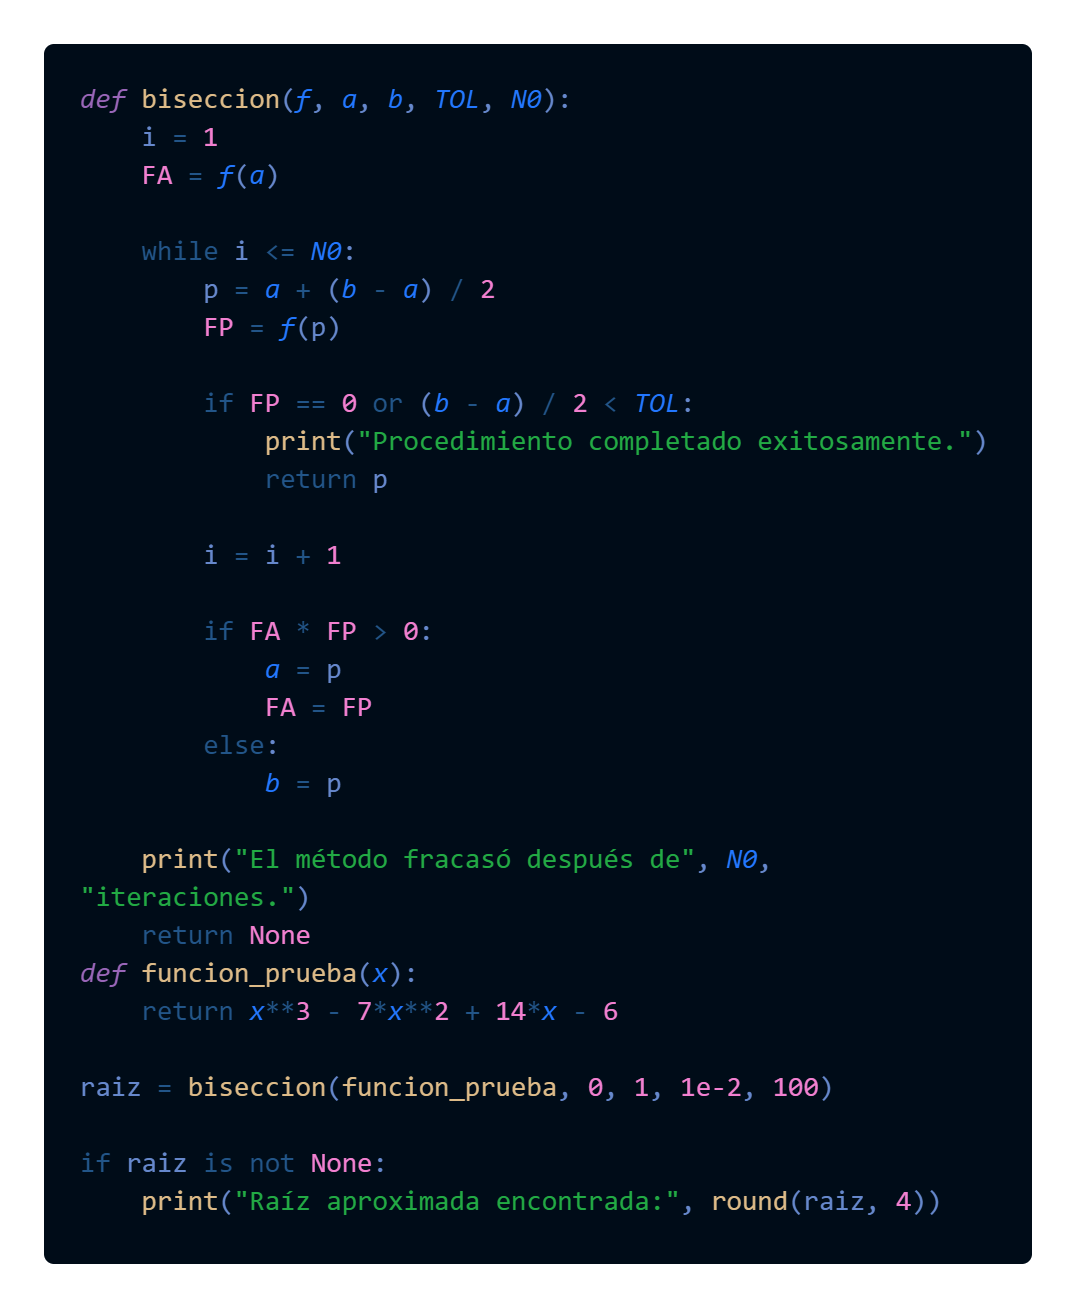
\includegraphics[width=0.75\textwidth]{inFiles/Figures/cdpsu.png}
\end{minipage}

\vspace{0.5cm}

\begin{minipage}{0.75\textwidth}
    \raggedleft
    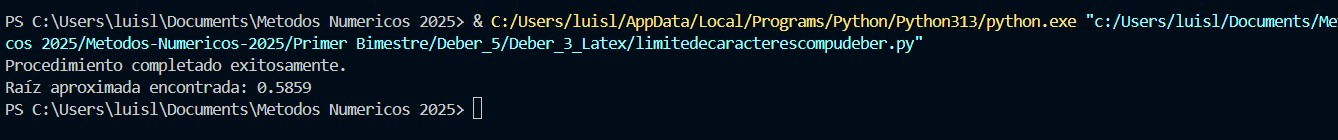
\includegraphics[width=0.75\textwidth]{inFiles/Figures/ejec1.jpg}
\end{minipage}

\vspace{0.5cm}

\begin{itemize}
\item {Use el método de bisección para encontrar soluciones precisas }
\end{itemize}

\begin{minipage}{0.75\textwidth}
    \raggedleft
    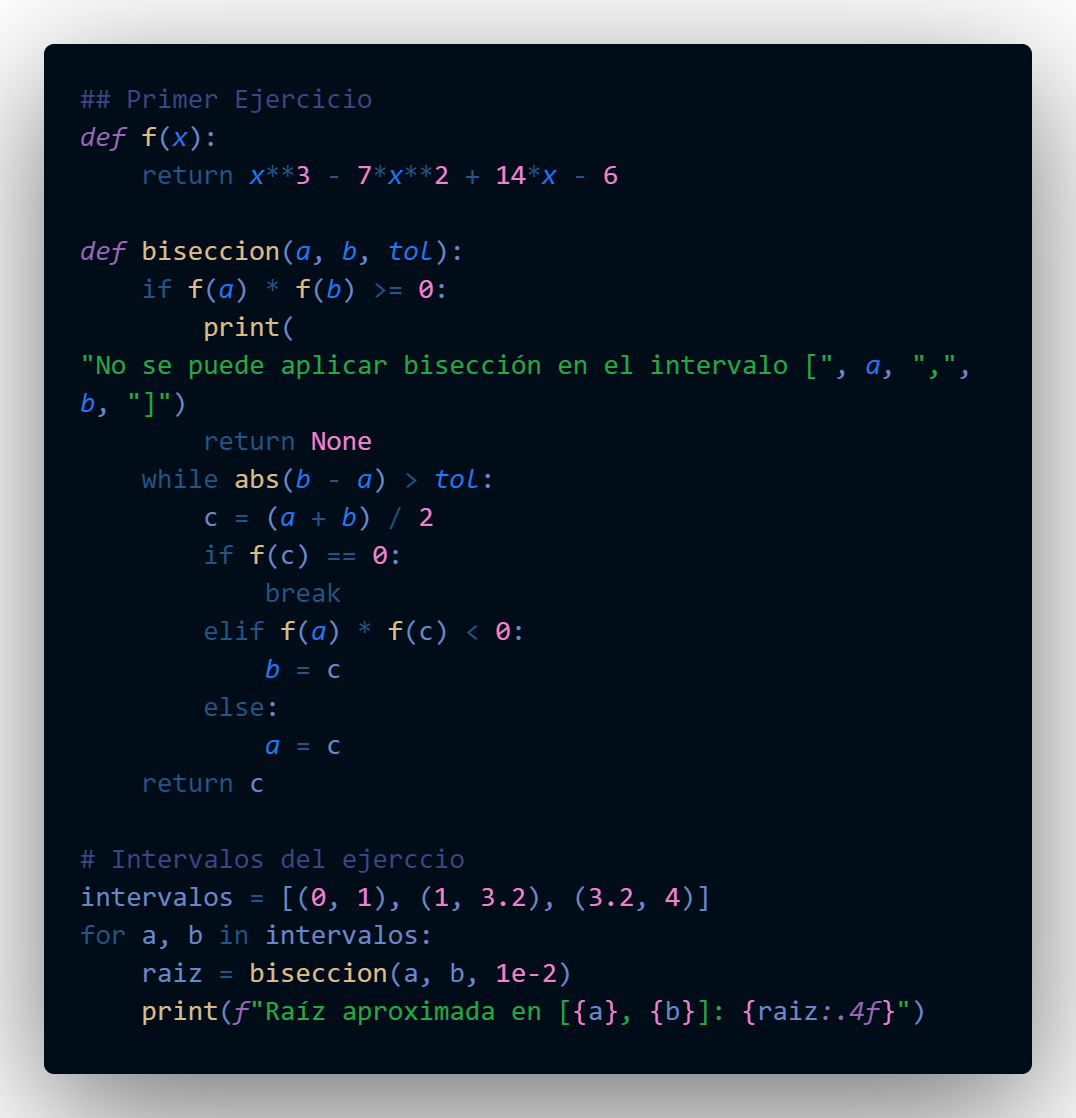
\includegraphics[width=0.75\textwidth]{inFiles/Figures/cd1.png}
\end{minipage}

\vspace{0.5cm}

\begin{minipage}{0.75\textwidth}
    \raggedleft
    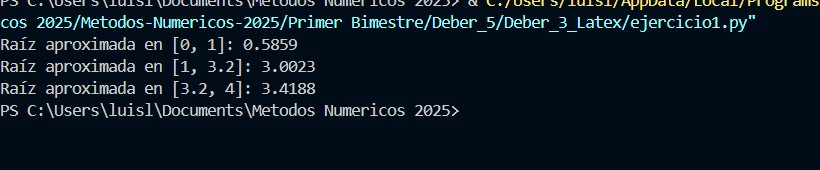
\includegraphics[width=0.75\textwidth]{inFiles/Figures/ejec2.jpg}
\end{minipage}

\vspace{0.5cm}

\begin{itemize}
\item {Dibuje las gráficas para y = x y y= sin x}
\end{itemize}

\begin{minipage}{0.75\textwidth}
    \raggedleft
    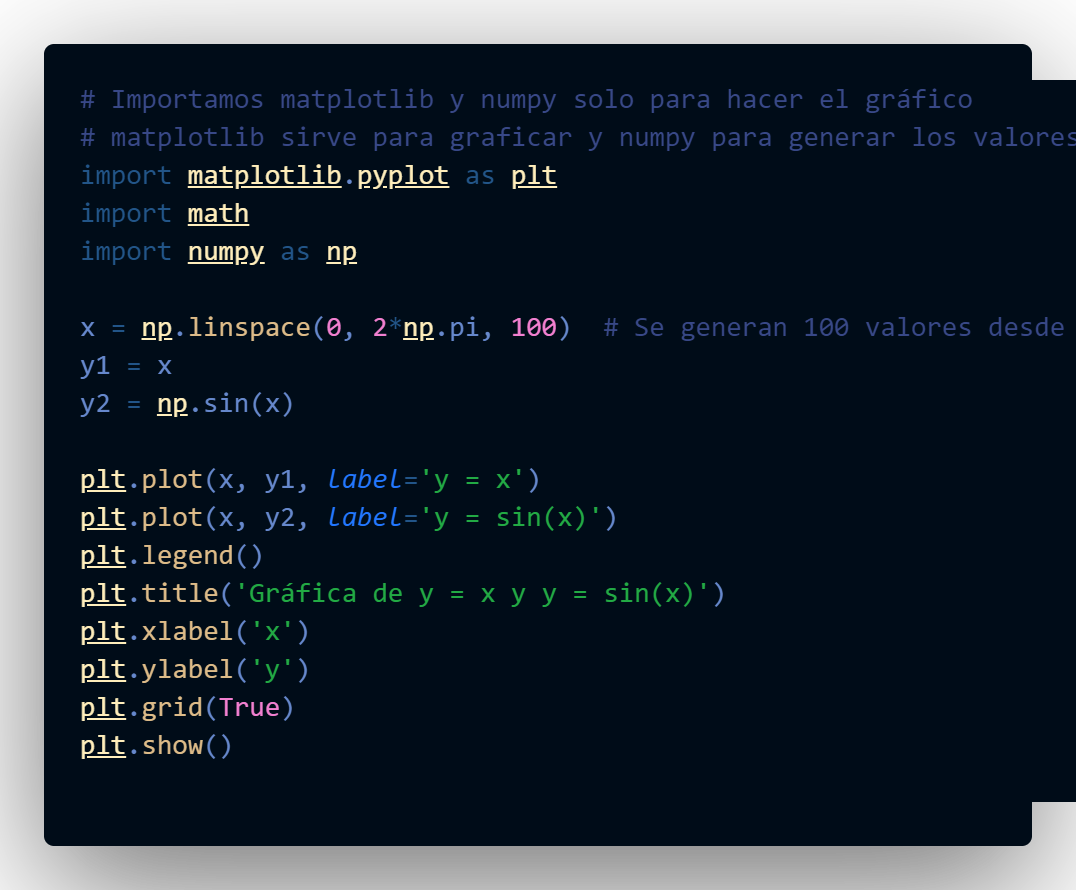
\includegraphics[width=0.75\textwidth]{inFiles/Figures/cd2.png}
\end{minipage}

\vspace{0.5cm}

\begin{minipage}{0.75\textwidth}
    \raggedleft
    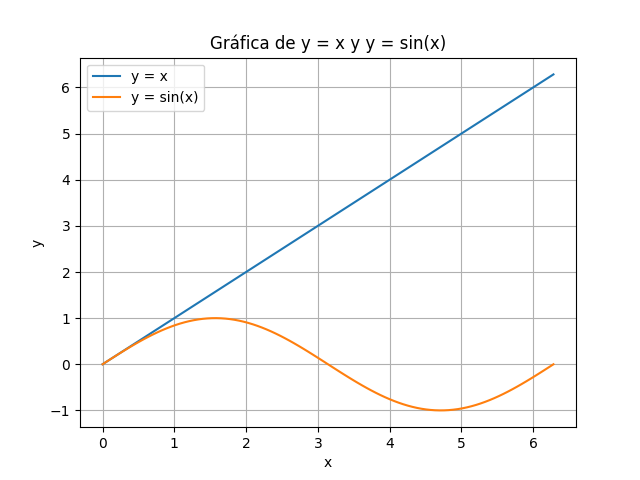
\includegraphics[width=0.75\textwidth]{inFiles/Figures/Graf_1.png}
\end{minipage}

\vspace{0.5cm}

\begin{itemize}
    \item {Use el método de bisección para encontrar soluciones precisas dentro de 10-5 para el primer valor positivo
    de x con x = 2 sin x}
    \end{itemize}

\begin{minipage}{0.75\textwidth}
    \raggedleft
    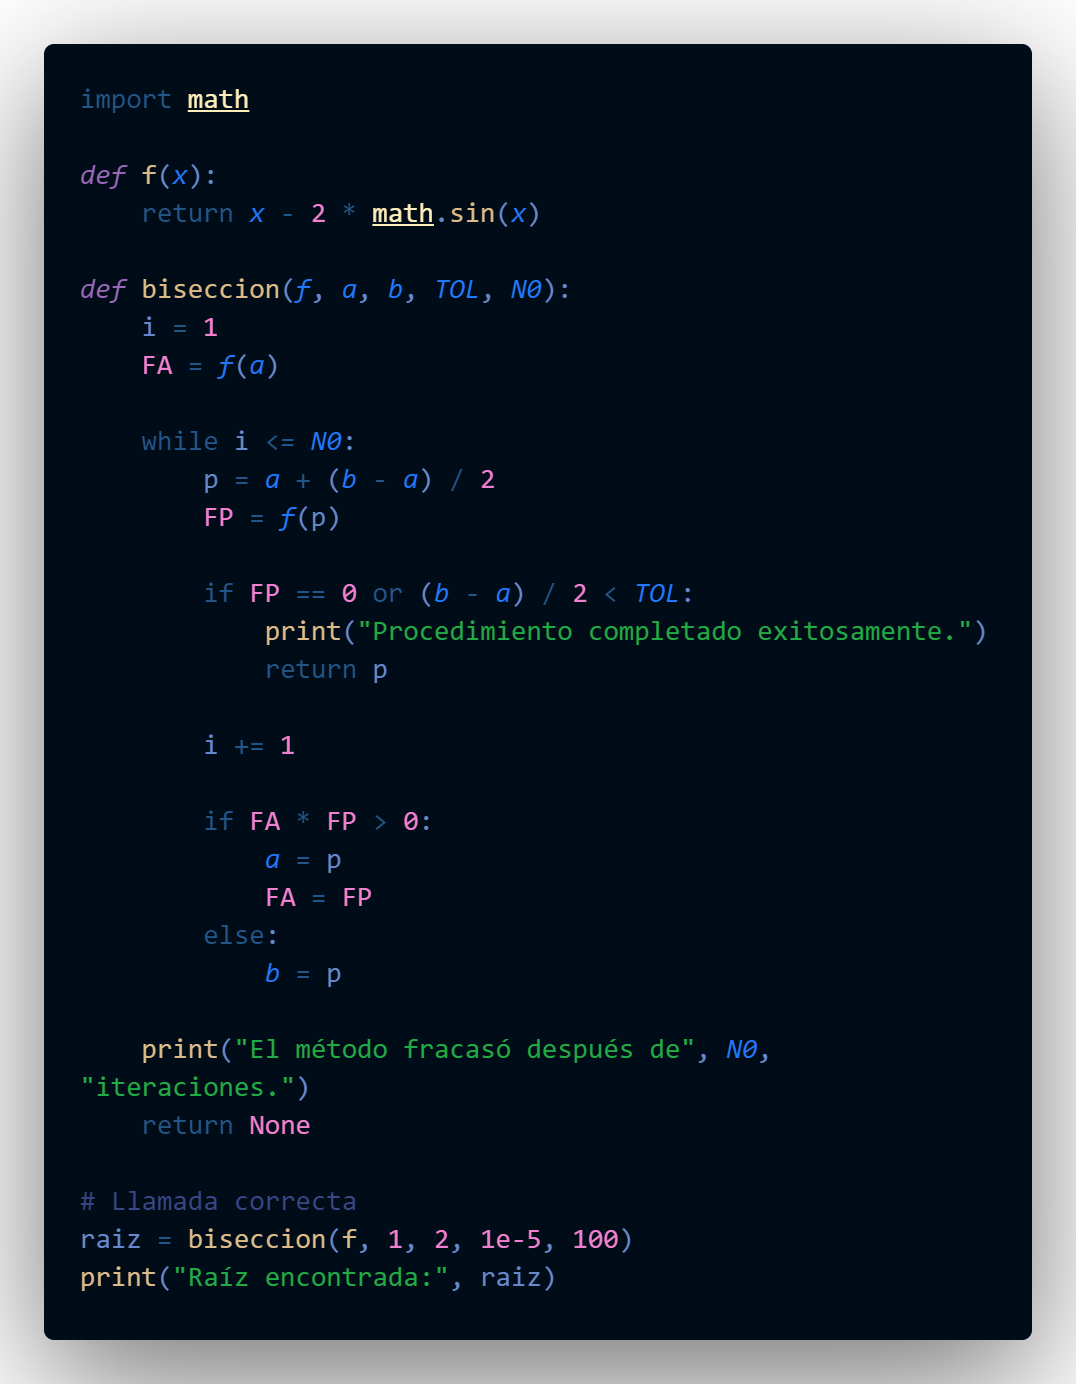
\includegraphics[width=0.75\textwidth]{inFiles/Figures/cd3.png}
\end{minipage}

\vspace{0.5cm}

\begin{minipage}{0.75\textwidth}
    \raggedleft
    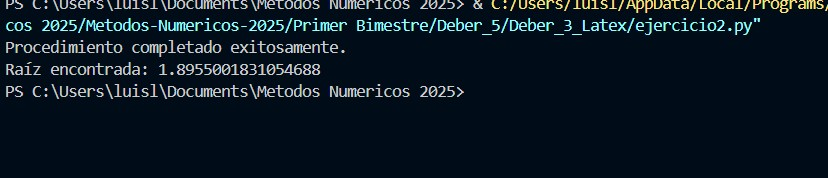
\includegraphics[width=0.75\textwidth]{inFiles/Figures/ejec3.jpg}
\end{minipage}

\vspace{0.5cm}

\begin{itemize}
    \item {Dibuje las gráficas para y = x y y = tan x}
    \end{itemize}

\begin{minipage}{0.75\textwidth}
    \raggedleft
    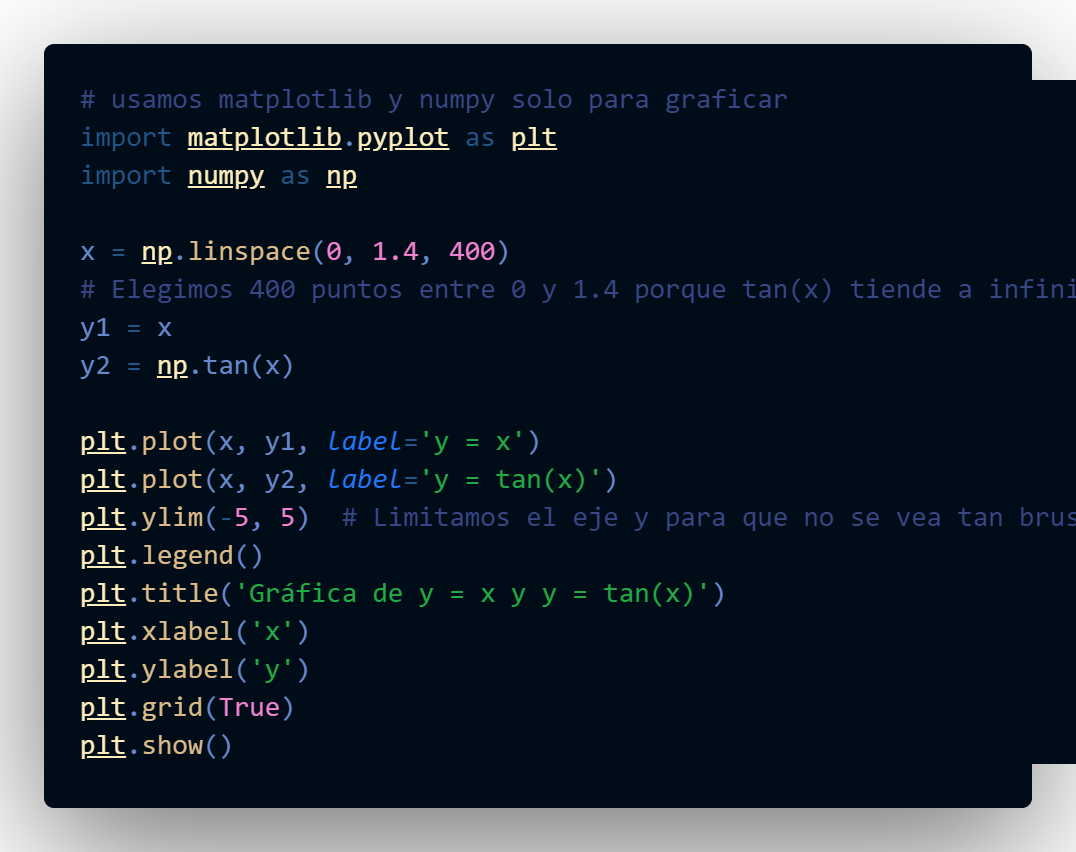
\includegraphics[width=0.75\textwidth]{inFiles/Figures/cd4.png}
\end{minipage}

\vspace{0.5cm}

\begin{minipage}{0.75\textwidth}
    \raggedleft
    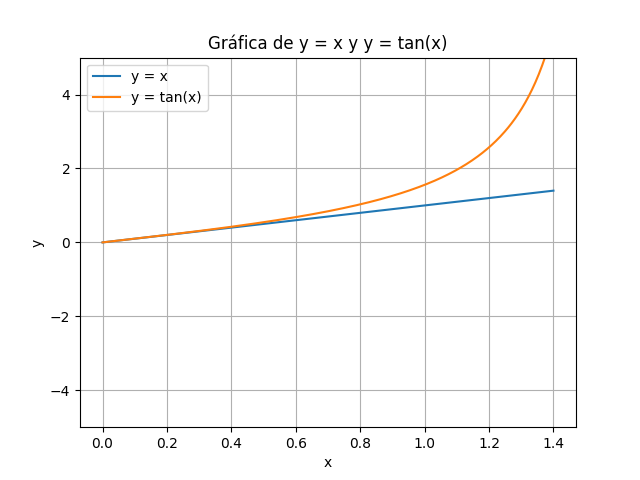
\includegraphics[width=0.75\textwidth]{inFiles/Figures/Graf_2.png}
\end{minipage}

\vspace{0.5cm}

\begin{itemize}
    \item {Use el método de bisección para encontrar una aproximación dentro de 10-5 para el primer valor positivo
    de x con x = tan x}
    \end{itemize}

\begin{minipage}{0.75\textwidth}
    \raggedleft
    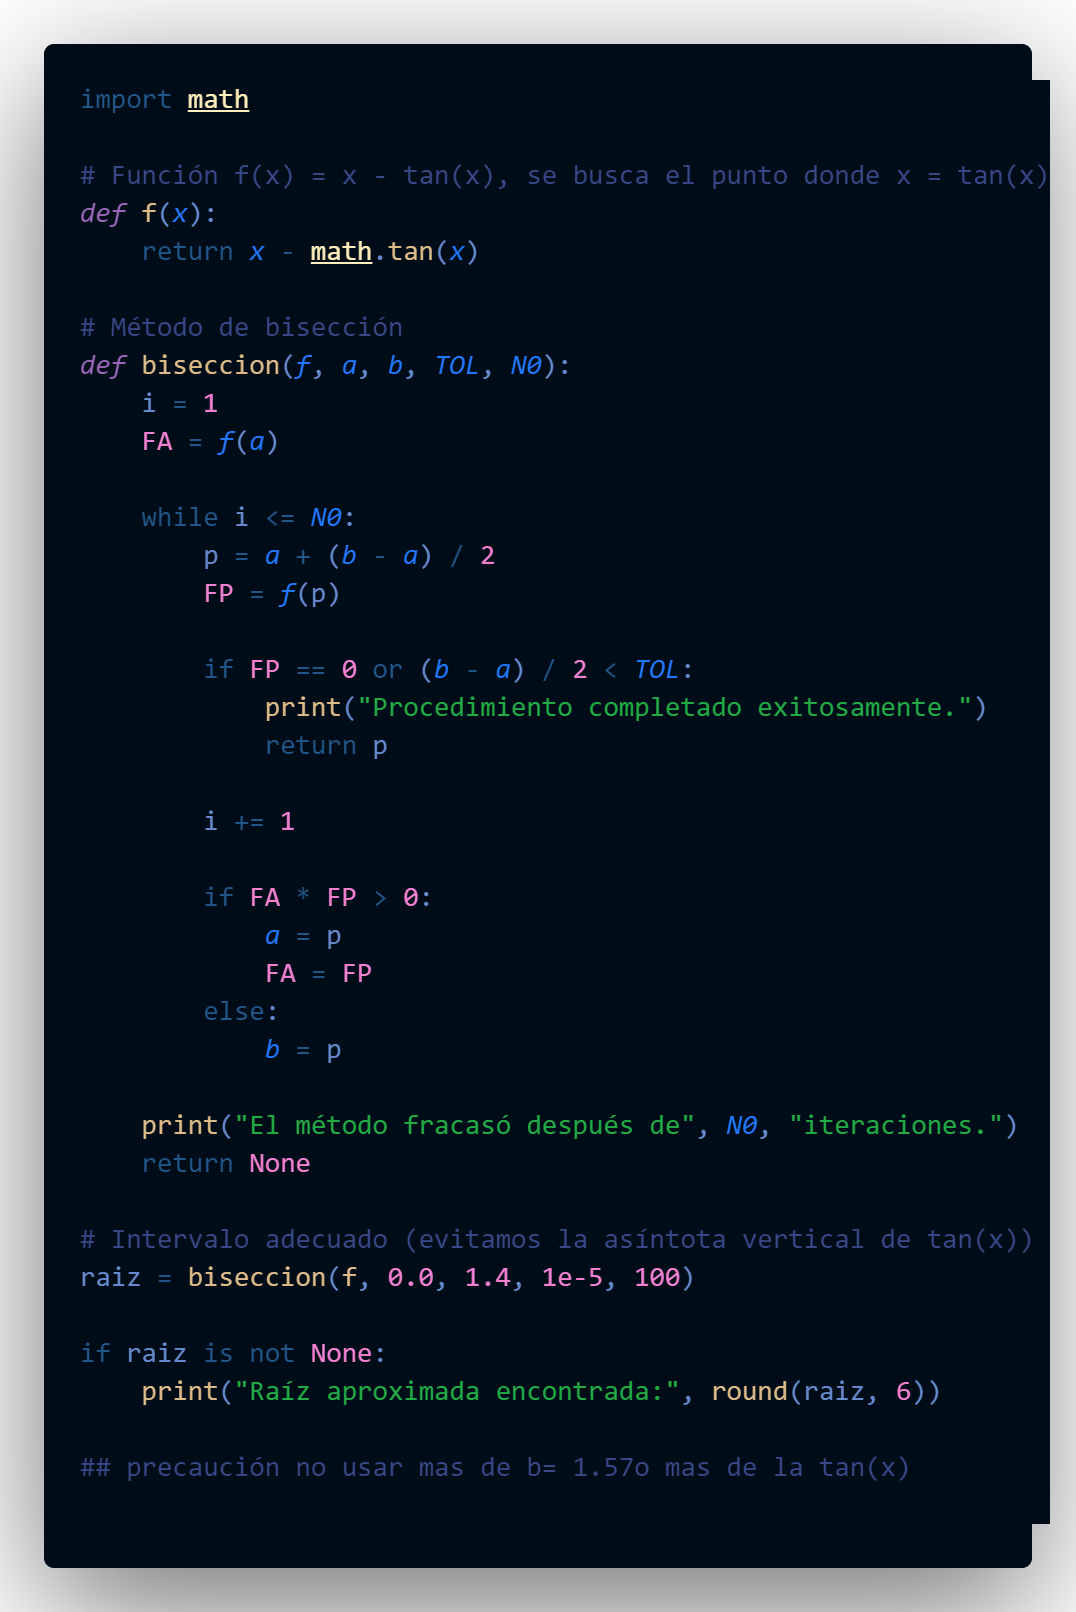
\includegraphics[width=0.75\textwidth]{inFiles/Figures/cd5.png}
\end{minipage}

\vspace{0.5cm}

\begin{minipage}{0.75\textwidth}
    \raggedleft
    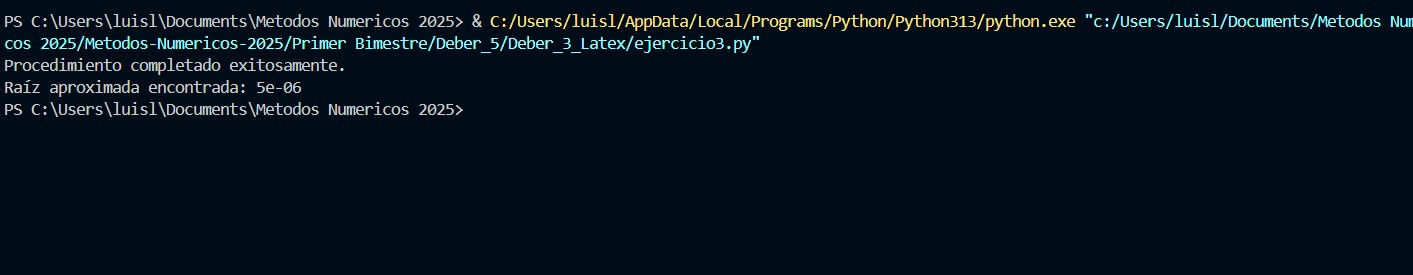
\includegraphics[width=0.75\textwidth]{inFiles/Figures/ejec4.jpg}
\end{minipage}

\vspace{0.5cm}


\begin{itemize}
    \item {Dibuje las gráficas para y = x^2-1 y y = e^1-x^2}
\end{itemize}

\begin{minipage}{0.75\textwidth}
    \raggedleft
    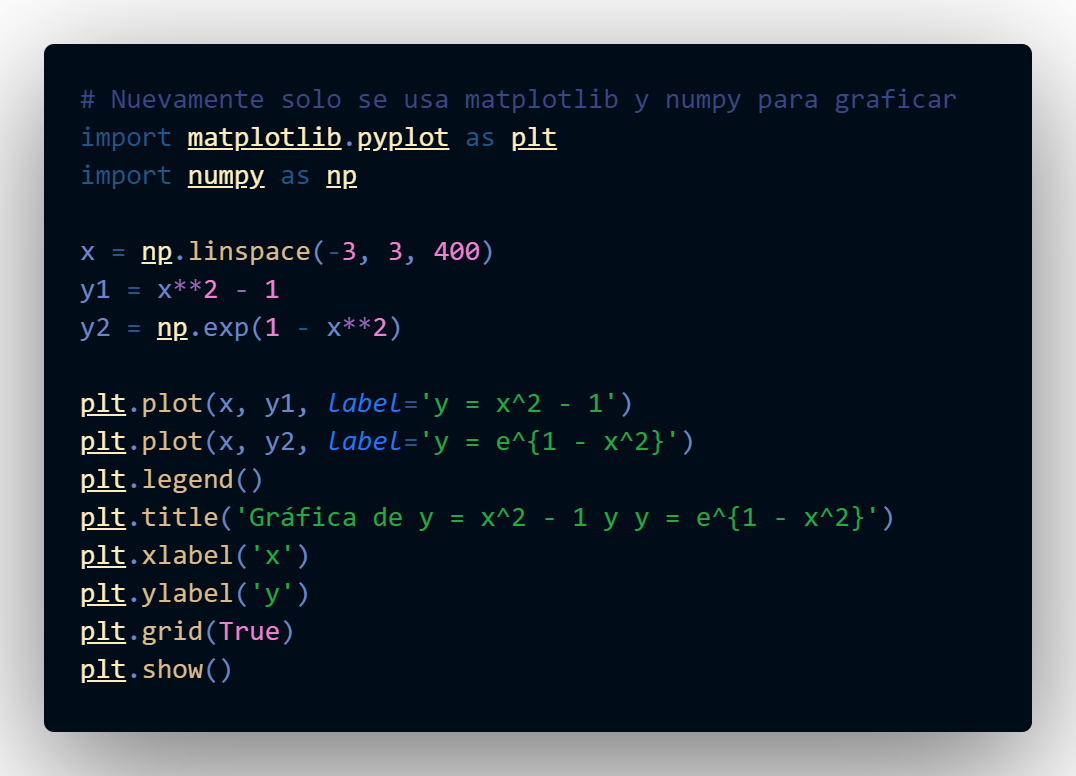
\includegraphics[width=0.75\textwidth]{inFiles/Figures/cd6.png}
\end{minipage}

\vspace{0.5cm}

\begin{minipage}{0.75\textwidth}
    \raggedleft
    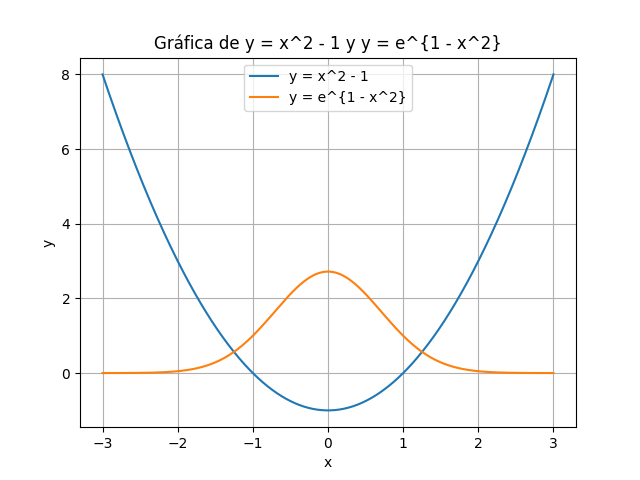
\includegraphics[width=0.75\textwidth]{inFiles/Figures/Graf_3.png}
\end{minipage}

\vspace{0.5cm}

\begin{itemize}
    \item {Use el método de bisección para encontrar una aproximación dentro de 10- para un valor  -2,0 
    con x^2-1=e^1-x^2}

\end{itemize}

\begin{minipage}{0.75\textwidth}
    \raggedleft
    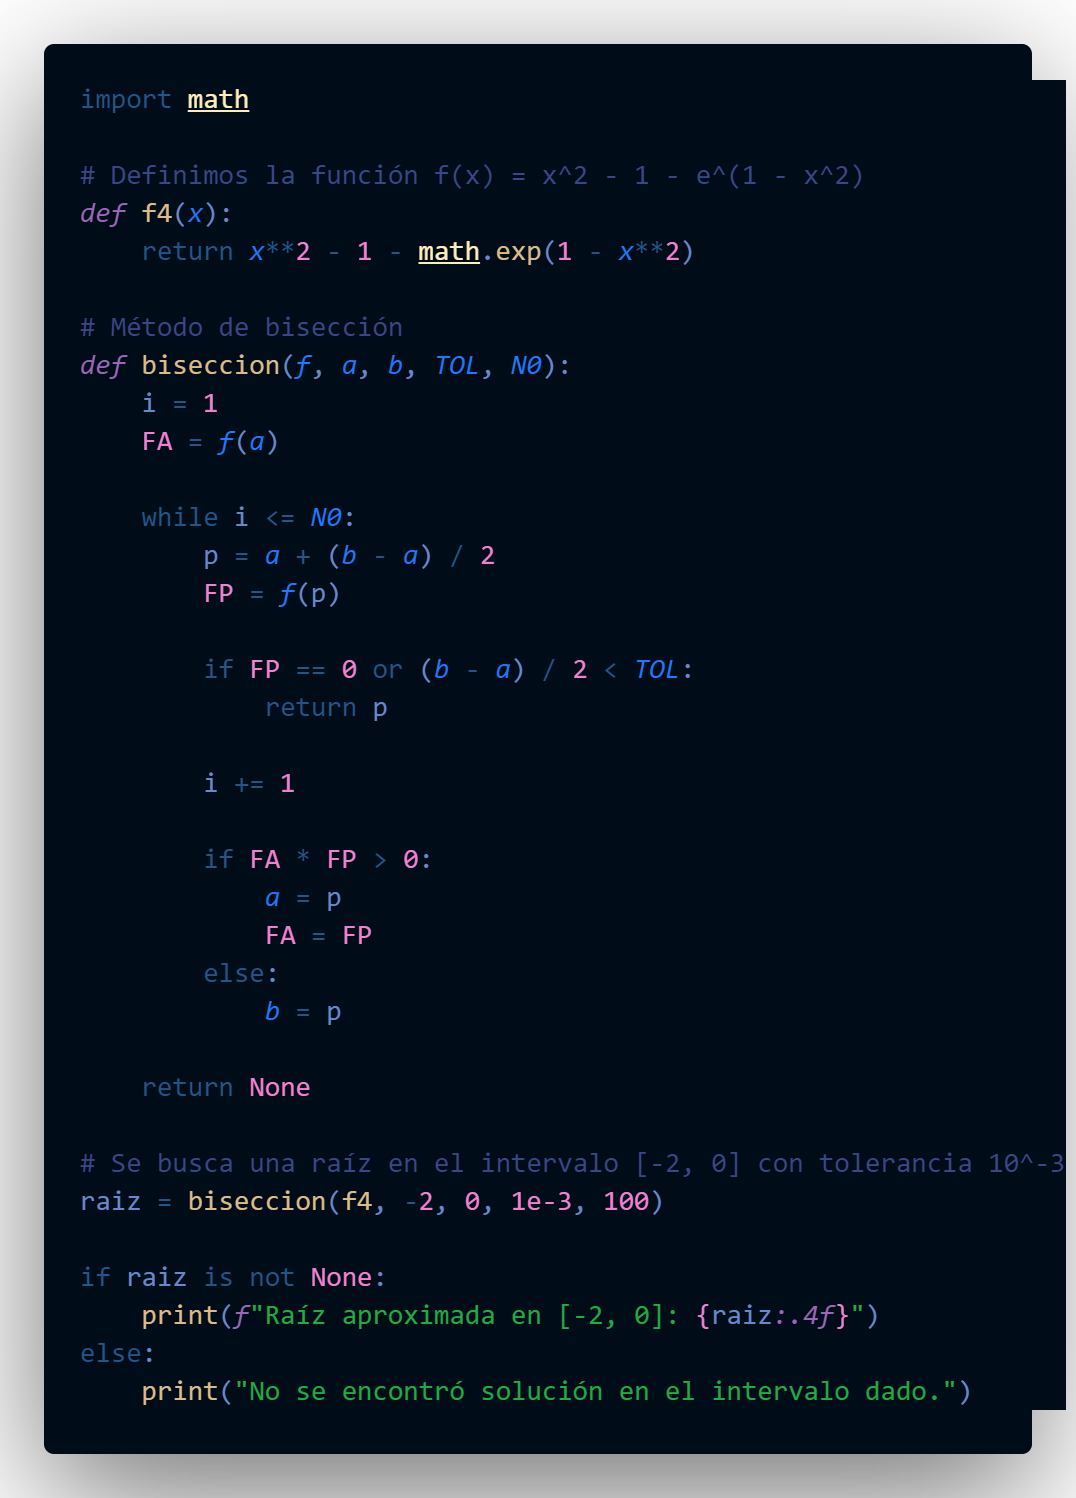
\includegraphics[width=0.75\textwidth]{inFiles/Figures/cd7.png}
\end{minipage}

\vspace{0.5cm}

\begin{minipage}{0.75\textwidth}
    \raggedleft
    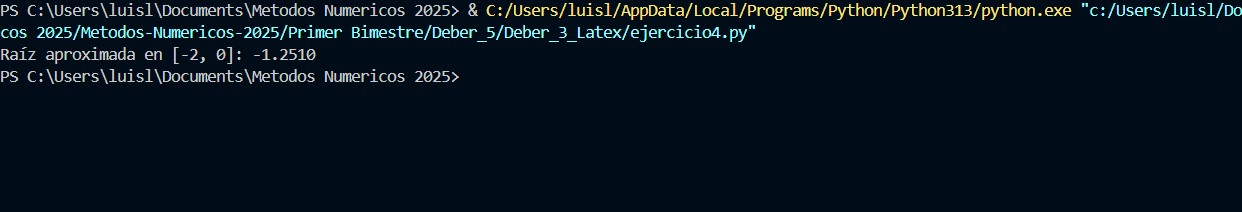
\includegraphics[width=0.75\textwidth]{inFiles/Figures/ejec5.jpg}
\end{minipage}

\vspace{0.5cm}

\begin{itemize}
    \item {Sea \( f(x) = \frac{(x + 2)(x + 1)^2 x (x - 1)^3}{(x - 2)} \). 
    ¿En qué cero de \( f \) converge el método de bisección cuando se aplica en los siguientes intervalos?
    }
    \end{itemize}

\begin{minipage}{0.75\textwidth}
    \raggedleft
    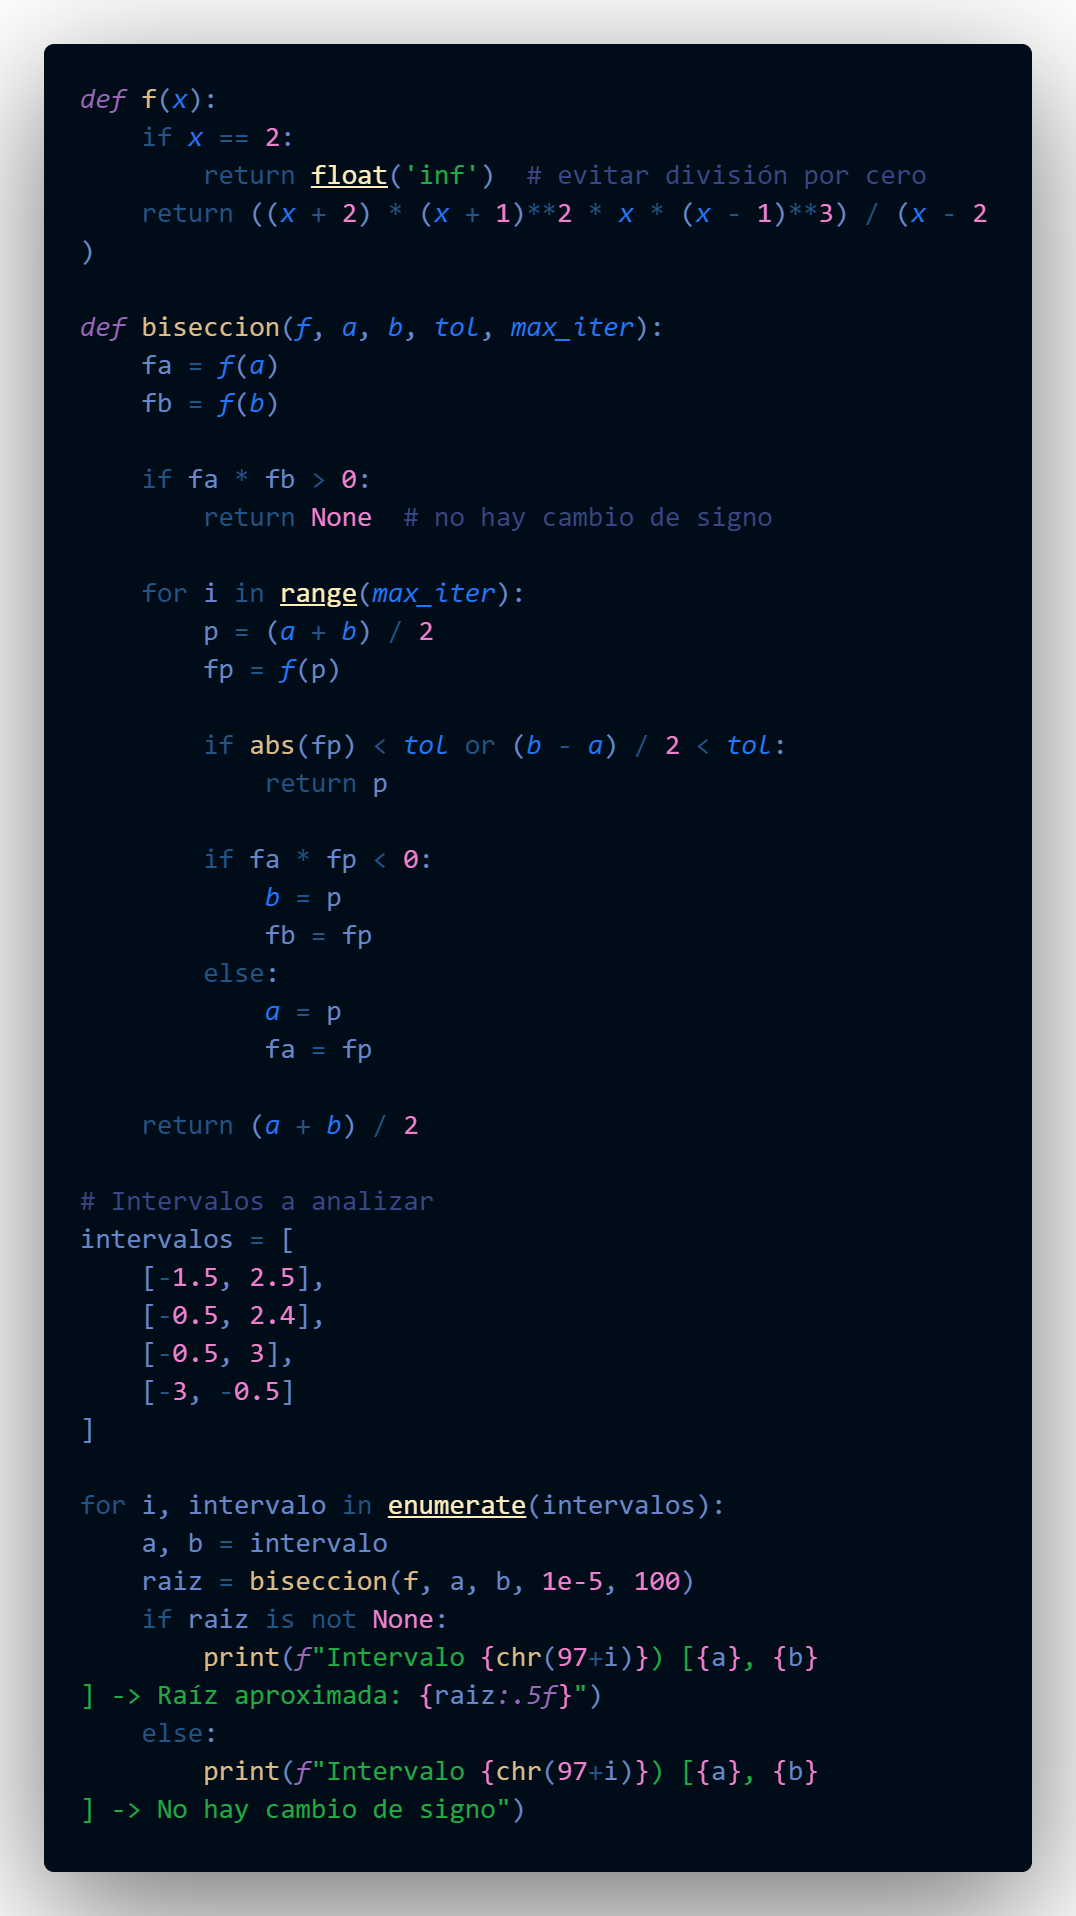
\includegraphics[width=0.75\textwidth]{inFiles/Figures/cd8.png}
\end{minipage}

\vspace{0.5cm}

\begin{minipage}{0.75\textwidth}
    \raggedleft
    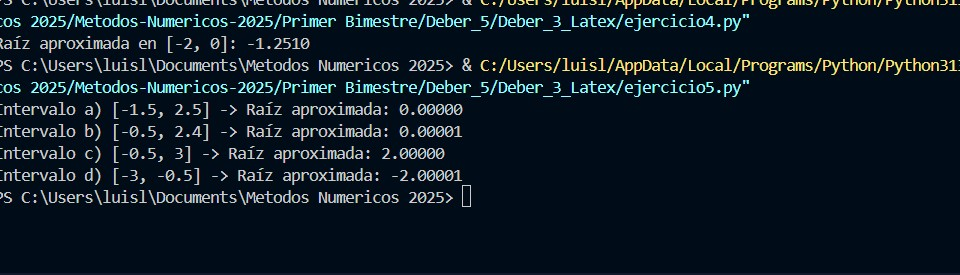
\includegraphics[width=0.75\textwidth]{inFiles/Figures/ejec6.jpg}
\end{minipage}

\vspace{0.5 cm}

\section*{CONCLUSIONES}
\begin{itemize}
    \item {El método de bisección funciona bien para encontrar raíces cuando la función cambia de signo en el intervalo.
     Aunque es un poco lento, es fácil de aplicar y da buenos resultados si se respetan las condiciones.}
\end{itemize}


\vspace{0.5cm}


\end{document}
